\chapter{Pre-Lab 2}
\setcounter{TASignatures}{0}
\setcounter{AsideCounter}{0}

\section{Introduction}

Make sure to complete this pre-lab before your assigned lab time. You will not be allowed to begin working on your lab without having this complete.

Each of the following problems are to be completed on paper. You are not expected to program these problems on PLC. You are expected to write neat ladder logic diagrams on paper.

\section{Background}


When you first start programming PLCs it is easy to mistakenly beleive the illusion that each rung is executed at the same time as if it really were an electrical circuit. This is \textbf{not} the case! The PLC scans the rungs in the ladder program from top to bottom and evaluates the instructions from left to right. Further, it processes branches within a rung top to bottom as well.

It is very important to consider the order in which things are scanned and how that will affect the outcome of the logic to be able to succeed in Lab 2.



\begin{figure*}[!b]
\centering
\textbf{Sequence that Forks}\par \medskip
\frame{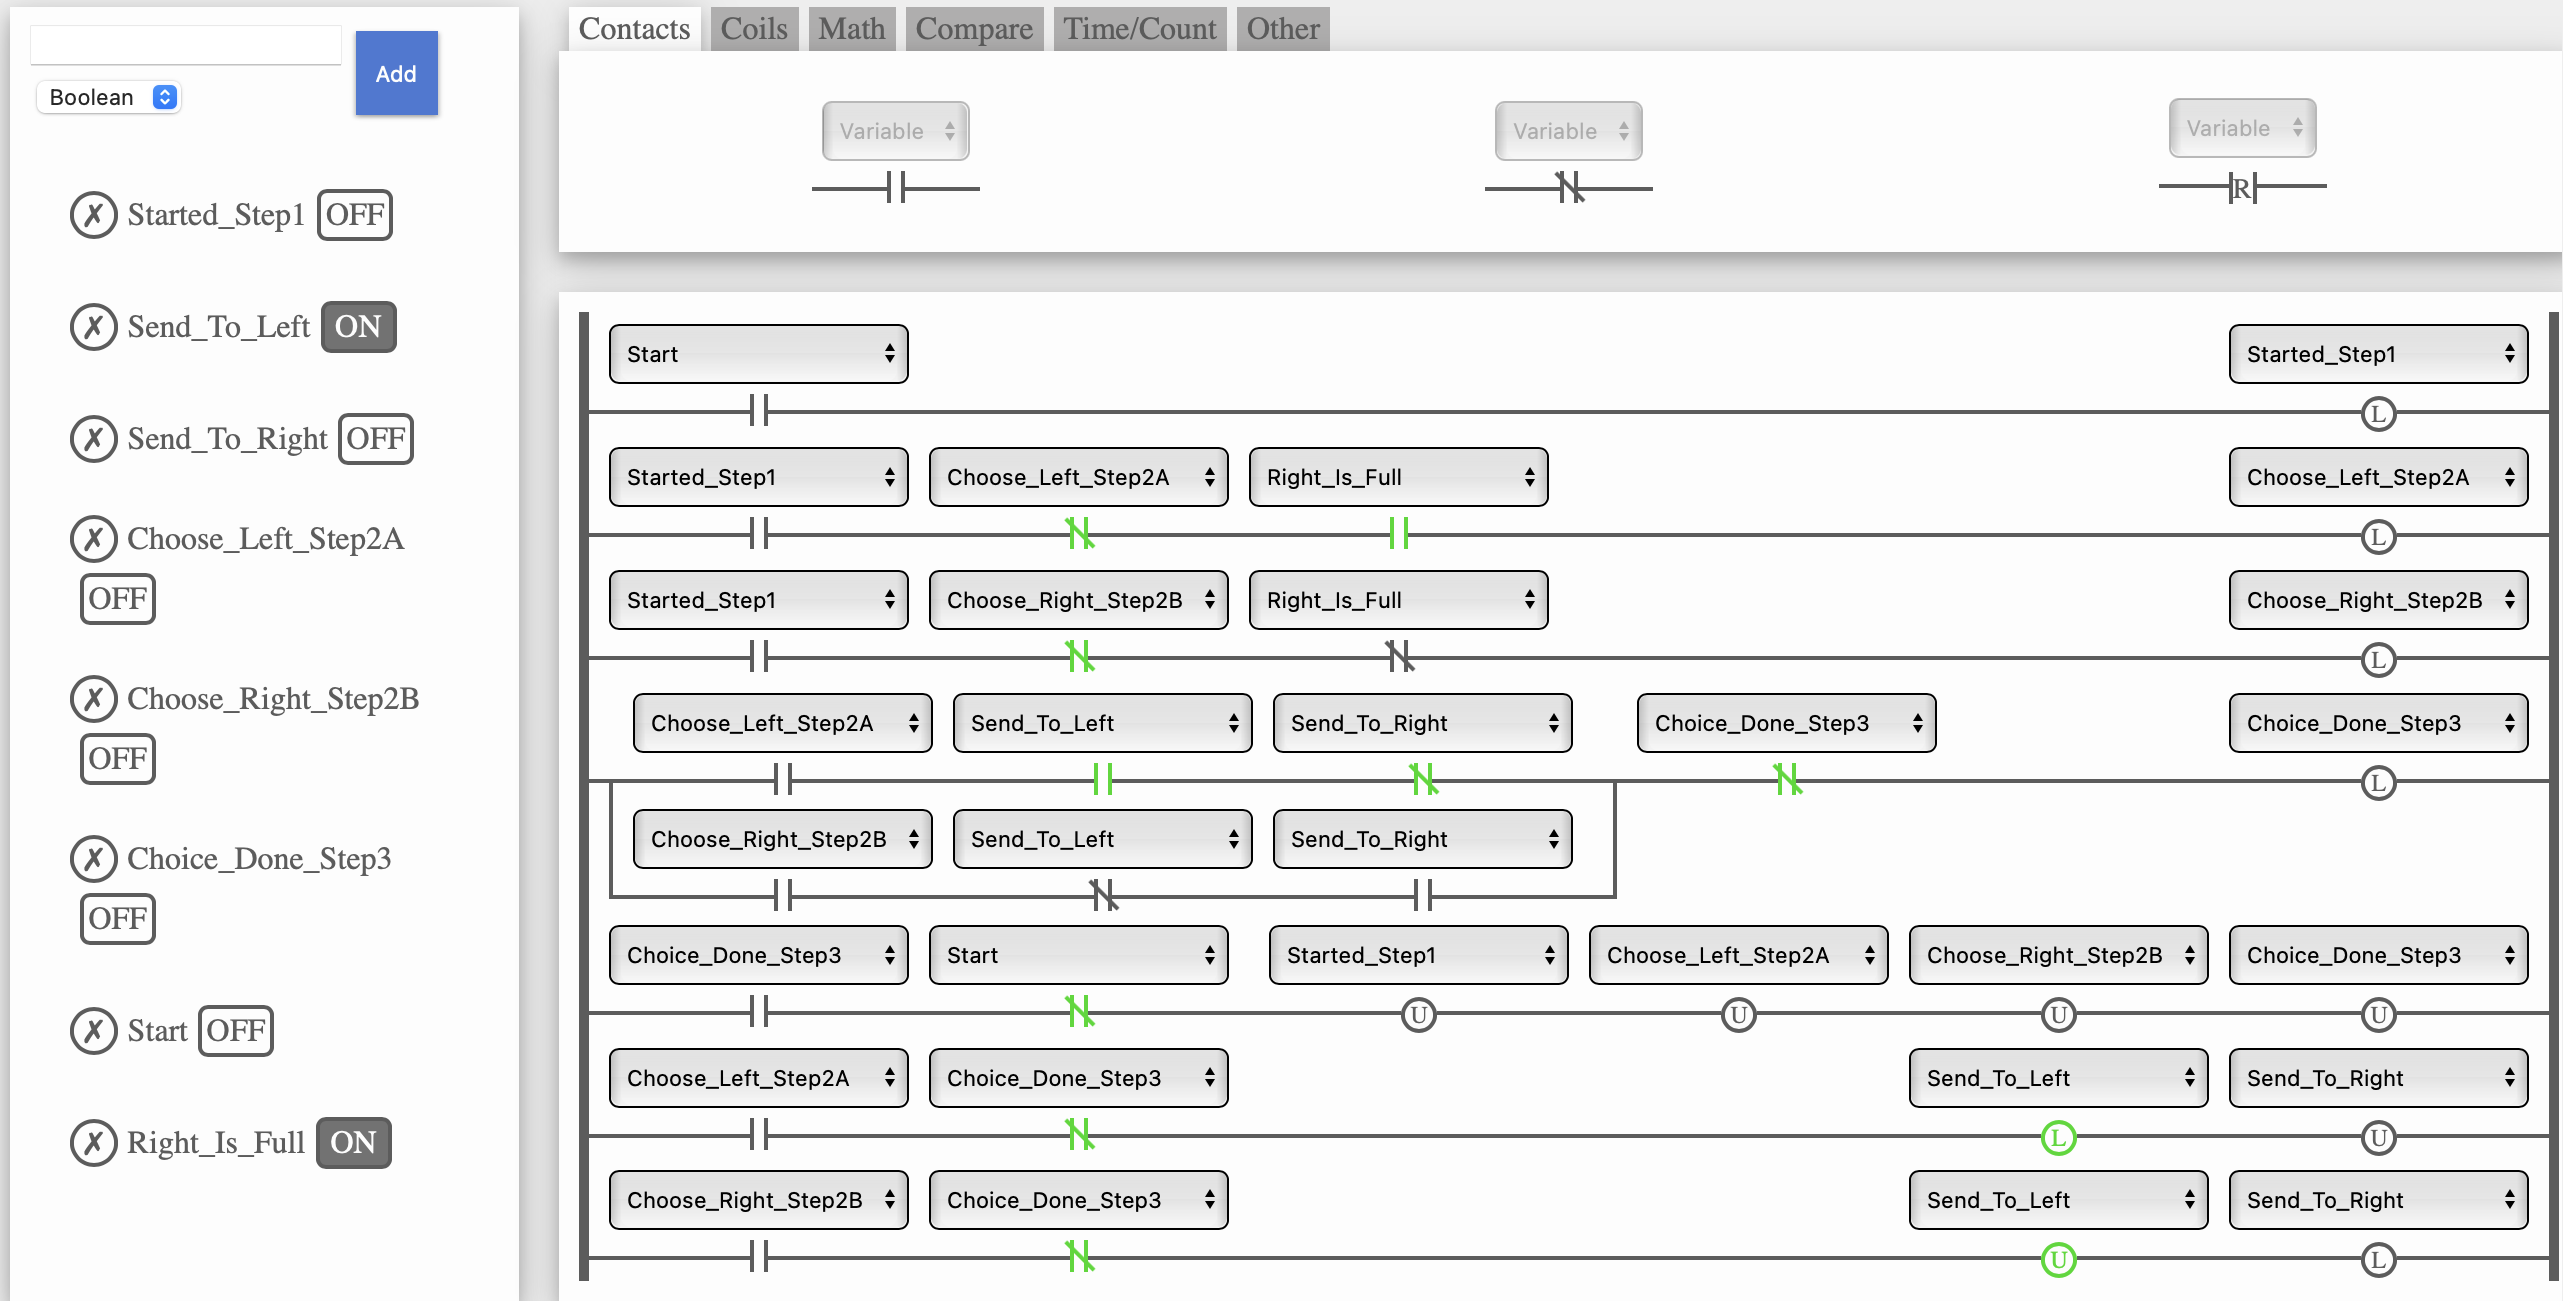
\includegraphics[width=0.9\paperwidth]{Images/Forking Sequence.png}}
\caption{Sequence with a Fork and Recombine}
\label{fig:ForkingSequence}
\end{figure*}

\section{Problem 1}

Write a simple bit latch sequence that will turn on the following boolean tags in order: \verb|turn_on_stove|, \verb|cook_food|, and \verb|turn_off_stove|. Your bit latch sequence should not move to the next step until the associated status bit comes on. So, after setting the tag \verb|turn_on_stove| to true, your sequence must wait for \verb|stove_is_on| to be true before moving to the next step. 

The signals your sequence turns on:
\verb|turn_on_stove|, \verb|cook_food|, and \verb|turn_off_stove|.

The feedback signals which allow you to move to the next step:
\verb|stove_is_on|, \verb|food_is_cooked|, and \verb|stove_is_off|.



\section{Problem 2}

The second problem is to write three rungs of ladder logic using the OTL and OTU instructions to toggle \verb|Toggle_Me| on the rising edge of the boolean tag \verb|change|. So, \verb|Toggle_Me| will change state every time \verb|change| goes from false to true. You are \textbf{not} allowed to use any instructions that have not been covered in class (NO oneshots!). You \textbf{are} allowed to use any and all instructions that have been covered and allowed to create extra boolean tags as necessary.


\subsection{Problem 2... Again}

The purpose of using bit latch sequencing (or any other structured programming) is two fold. First, it is very helpful to have a structure to your path forward to limit the world of possible solutions. But, secondly and most important, using a structured approach to programming allows others to anticipate and easily understand your code.

Solve the toggle problem described previously using a bit latch sequence. You may use up to six rungs of ladder logic. To accomplish this, you will need to have create a fork in the sequence. Then after some action, you can recombine. To make this more clear, refer to the image in \ref{fig:ForkingSequence}


\section{Problem 3}

Write \textbf{two rungs} of ladder logic to implement the challenge boolean formula from lab 2: $D = \overline{((A+B)\cdot C\cdot A)}$. Do, not use Demorgan's theorem to change the form of the equation. Rather, approach the problem in a manner similar to that shown in the sequential logic in \figureautorefname \ref{fig:Problem3_pl2}.

\lstset{style=mystyle}
\lstset{language=python}
\begin{figure}[h]
\begin{lstlisting}[firstnumber=1]

while(True){
    if((A or B) and C and A):
        Temporary_Tag = True
    else:
        Temporary_Tag = False
        
    if(Temporary_Tag):
        D = False
    else:
        D = True
}
    
\end{lstlisting}
\caption{Pre-lab problem 3}
\label{fig:Problem3_pl2}
\end{figure}

\section{Problem 4 - Read the Manual}

Read the lab manual. Then write a paragraph about the content and expectations in the lab manual which will convince the grader that you have in fact read the complete lab manual.